\begin{figure}[tb]
  \centering
  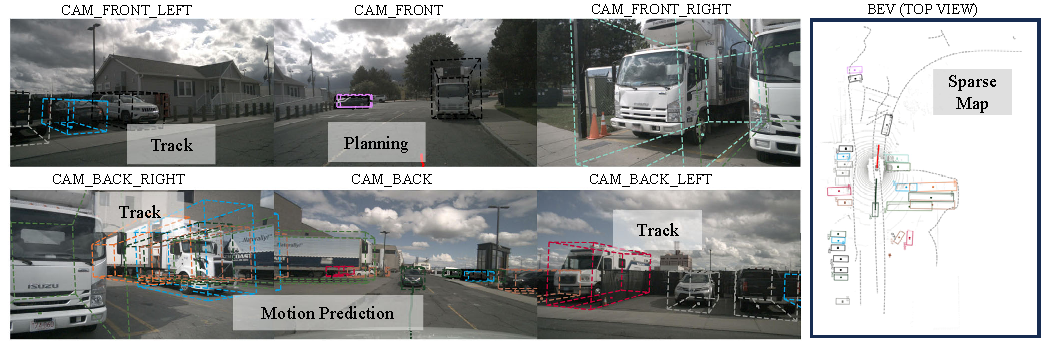
\includegraphics[width=1\linewidth]{Figures/Visualization-Figure}
  \caption{定性可视化。在环视图像和BEV中绘制所有任务的结果。每个智能体在图像和BEV中均以不同颜色的虚线边界框标记。地图元素的稀疏预测仅以灰色虚线在BEV中显示。分别选择运动预测的top-1模态和自车规划结果在图像和BEV上进行可视化。BEV中的激光雷达点云仅用于可视化，不作为模型输入。}
  \label{fig:vis}
\end{figure}